\subsection{Participants}
In total, there were 45 available cases.
Most cases were concerned with pilocytic astrocytoma (17) and medulloblastoma (8).
This amounts to a total of 134 images of which are 26 overview images and 108 close-up images.
These cases were included in the training and testing of the model.
The included images were taken between 26 September 2022 and 13 April 2023.
No participants have received prior treatment and no images of follow-up treatments are included.

\begin{table}
    \caption[Number of cases per diagnosis]{
        Number of cases per diagnosis.
        Bold rows were included in this study.
    }
    \label{tab:available_data}
    \begin{tabular}{lr}
        \toprule
        Diagnosis &  Count \\
        \midrule
        \textbf{Pilocytic astrocytoma}               &         \textbf{17} \\
        \textbf{Medulloblastoma}                     &          \textbf{8} \\
        Craniopharyngioma                   &          5 \\
        Ganglioglioma                       &          3 \\
        Ependymoma                          &          1 \\
        Glioma                              &          1 \\
        Medulloblastoma                  &          1 \\
        Diffuse midline glioma              &          1 \\
        Dysembryoplastic neuroepithelial tumor  &          1 \\
        Pituitary Neuroendocrine Tumors               &          1 \\
        Atypical choroid plexus papilloma   &          1 \\
        Neuroendocrine tumor                &          1 \\
        Infantile hemispheric glioma        &          1 \\
        Subependymal giant cell astrocytoma &          1 \\
        Reactive                            &          1 \\
        No neoplasm                         &          1 \\
        \bottomrule
    \end{tabular}
\end{table}

The age and sex of the subjects per fold are summarized in \cref{fig:age-and-sex-diagnosis}.

\begin{figure*}
    \centering
    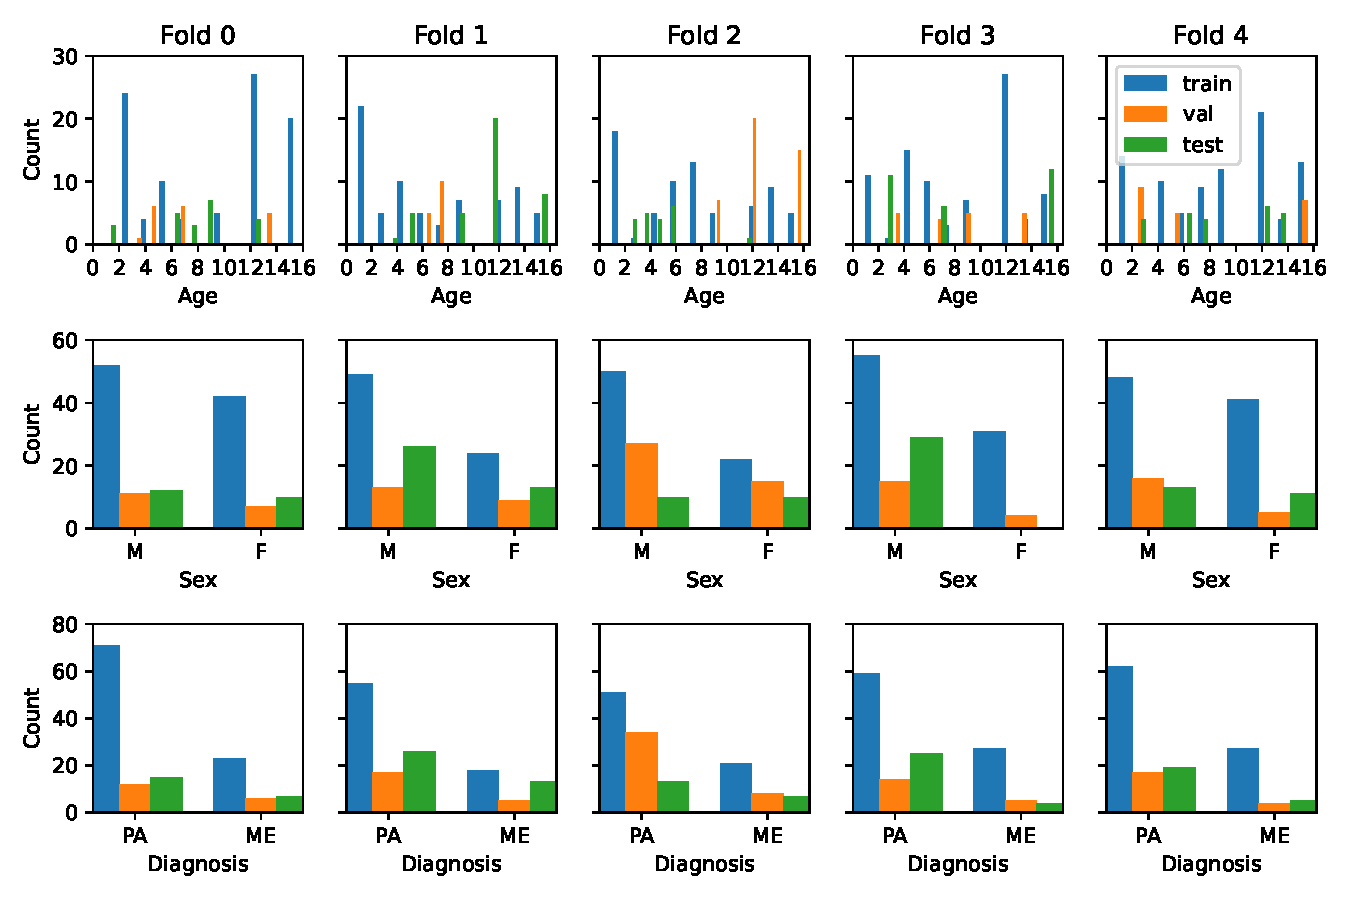
\includegraphics[width=\linewidth]{pediatric-brain-tumours/images/age-and-sex-diagnosis-per-fold.pdf}
    \caption[Age and sex distribution]{Age, sex, and diagnosis distribution per training, validation and test split for every fold.
    Only pilocytic astrocytoma (PA) and medulloblastoma (ME) cases are included.}
    \label{fig:age-and-sex-diagnosis}
\end{figure*}